% !TEX root = thesis.tex

\section{Discussion}
\label{sec:disc}
\cite{Chatrchyan:2014gia,Dasgupta:2007wa}

\subsection{Dihadron \texorpdfstring{$\jt{}$}{jT}}
The jet fragmentation transverse momentum $\jt{}$ has been studied previously at ALICE with dihadron correlations~\cite{ALICEjt}. The study took the leading hadron in each event and calculated $\jt{}$ for any near-side tracks with respect to the leading hadron. Thus there is no kinematical limit to $\jt{}$ from the jet cone. In the analysis the background shape is estimated using pairs with large $\Delta \eta$. The normalisation of the background is done when fitting the $\jt{}$ distribution. The inclusive and signal distributions from the analysis are shown in Fig.~\ref{fig:dihadron}. The inclusive distribution is fitted with a three component function, 

\begin{figure}[htp]
\centering
\begin{subfigure}{0.49\textwidth}
\includegraphics[width = 0.95\textwidth]{pics/jtdistribution-89702.pdf}
\end{subfigure}
\begin{subfigure}{0.49\textwidth}
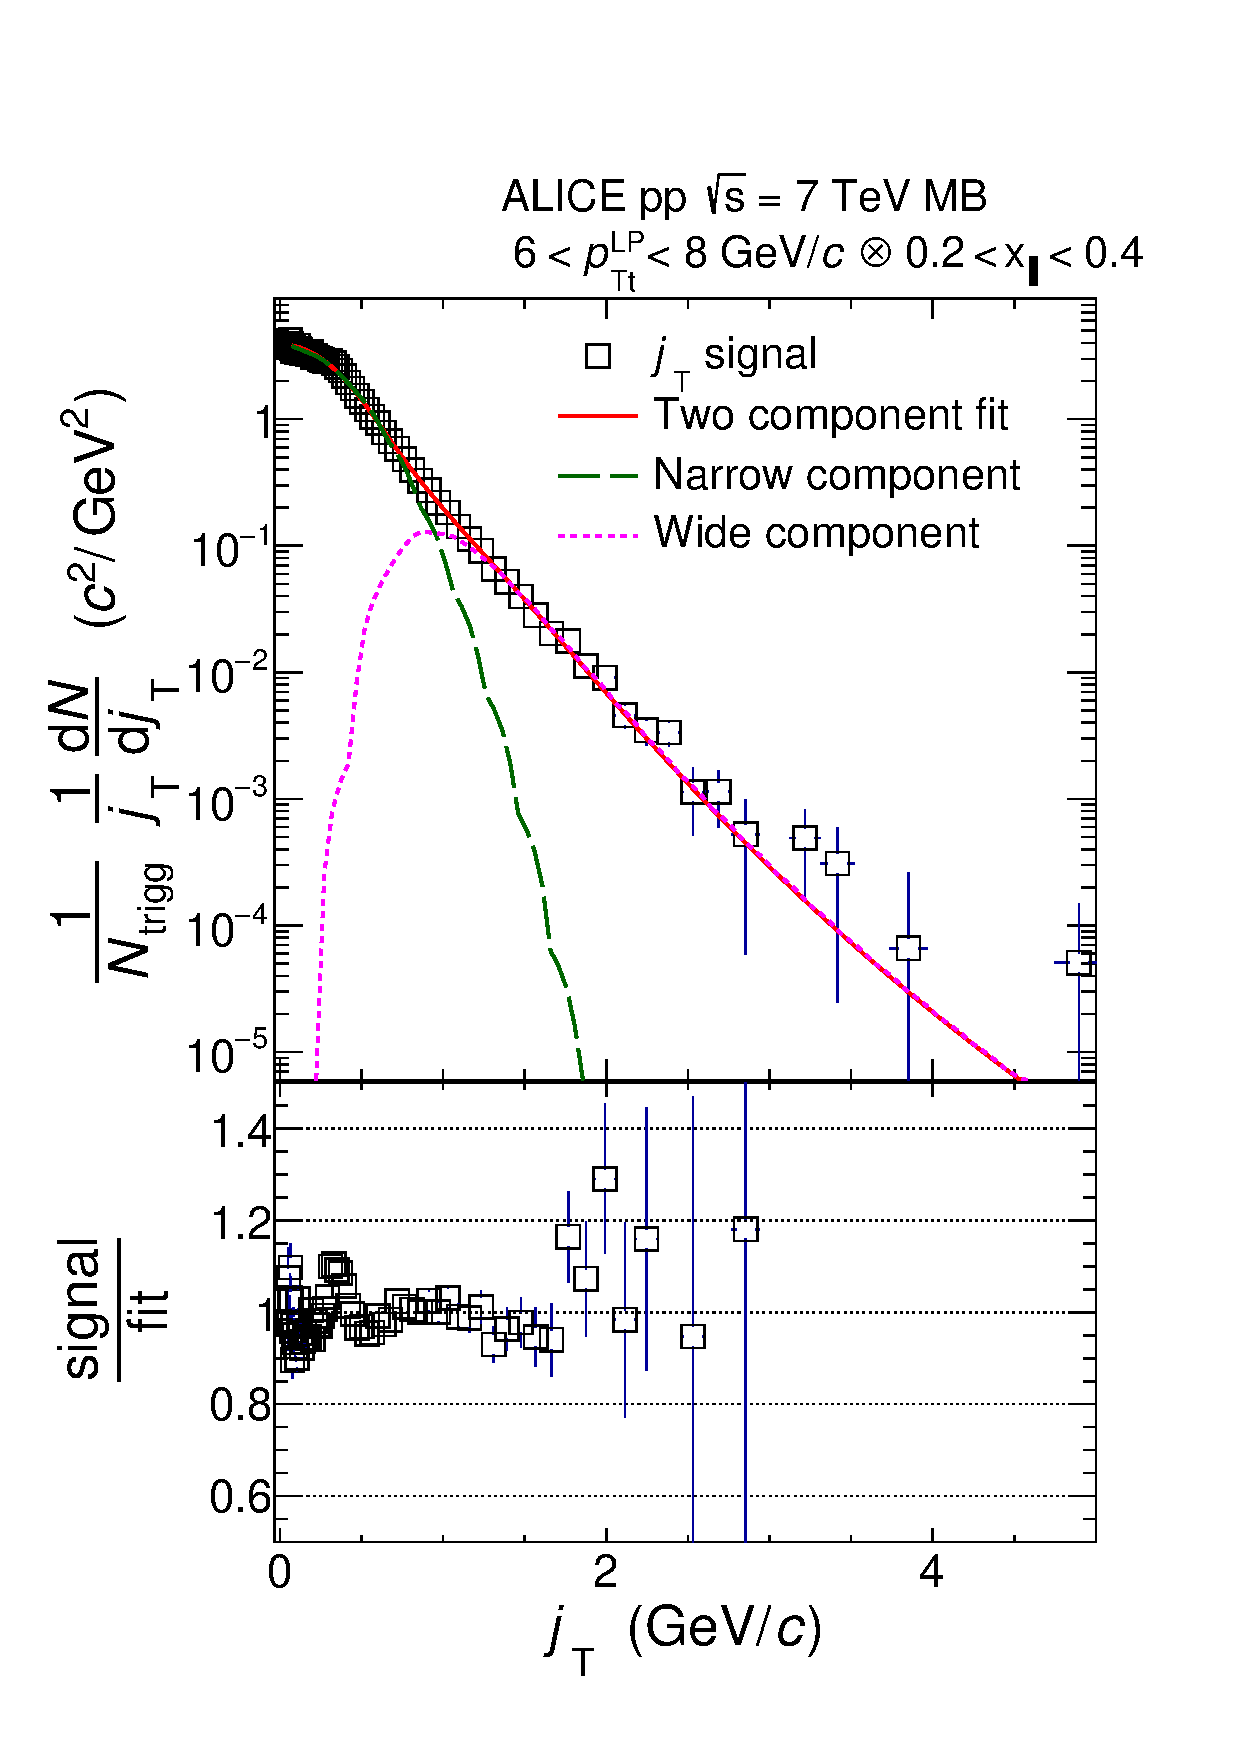
\includegraphics[width = 0.95\textwidth]{pics/jtsignal-89703}
\end{subfigure}
\caption[Dihadron $\jt{}$ results]{\emph{Left:} Measured \jt distribution including a three-component fit. The three components describe the background (circular symbols), hadronization (long dashed line), and showering (short dashed line). \emph{Right:} The same \jt distribution but with background subtracted.}
\label{fig:dihadron}
\end{figure}


%\begin{multline}
%\mathrm{Constant\:\times\:background\:+\:Gauss\:+\:Inverse\:Gamma} \\
%B_0 \times\:\mathrm{background} + \frac{B_2}{B_1\sqrt{2\pi}}e^{-\frac{\jt{}^2}{2B_1^2}}+\frac{B_3B_5^{B_4}}{\Gamma\left(B_4\right)}\frac{e^{-\frac{B_5}{\jt{}}}}{\jt{}^{B_4+1}}.
%\end{multline

The analysis was the first to introduce this factorisation of $\jt{}$ into components.

At $\jt{} \approx 0.4 \gev$ there is a small bump in the distribution to fit ratio. This was attributed to cases where the trigger particle decayed after hadronisation. As it is difficult to correct for, this bump is included in the systematic errors of the results.  


The RMS results from the fitting in both \pp and \pPb collisions are shown in Fig.~\ref{fig:dihadronResults}. Qualitatively the results are similar to jet $\jt{}$ results. The RMS value of the wide component has an increasing trend with respect to $\pt{t}/\pt{jet}$, while the RMS value of the narrow component stays constant. Both components are well described by \pythia~simulations. As seen in the figures there is no difference between \pp and \pPb results in the dihadron analysis. 



\begin{figure}[htb]
\centering
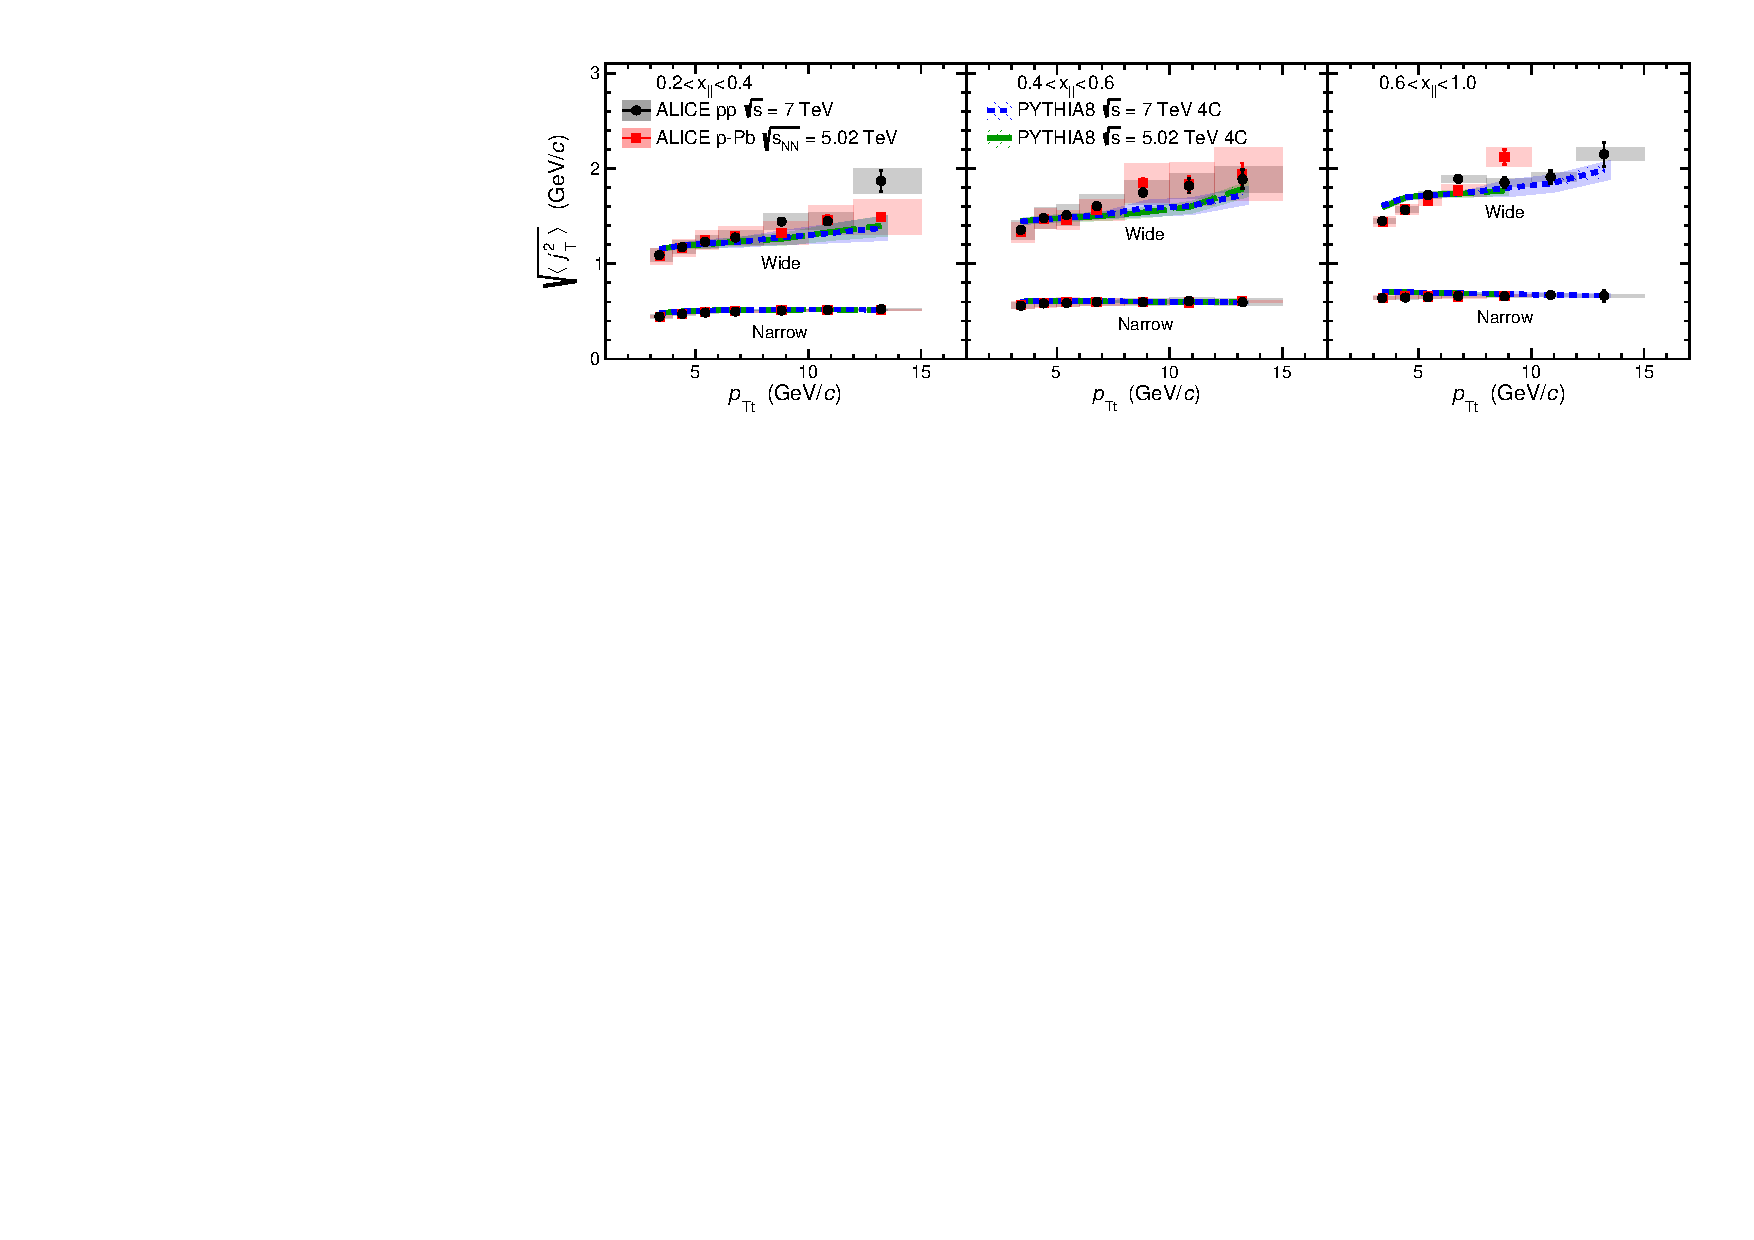
\includegraphics[width=0.95\textwidth]{pics/jt_RMS_finalFormUniformTextSize-89708}
\caption{RMS values of the narrow and wide $\jt{}$ components in the dihadron correlation analysis. Results from \pp collisions at $\sqrt{s} = 7 \tev$ (circular symbols) and from \pPb collisions at \sqrtSnnE{5.02} (square symbols) are compared to \textsc{Pythia}~8 tune 4C simulations at \sqrtSE7 (short dashed line) and at \sqrtSE{5.02} (long dashed line). Different panels correspond to different \xlong bins with 0.2<\xlong<0.4 on the left, 0.4<\xlong<0.6 in the middle, and 0.6<\xlong<1.0 on the right. The statistical errors are represented by bars and the systematic errors by boxes.~\cite{ALICEjt}}
\label{fig:dihadronResults}
\end{figure}


\subsection{Comparing dihadron and jet \texorpdfstring{$\jt{}$}{jT} results}
Comparison to RMS values in dihadron analysis~\cite{ALICEjt} are shown in figure \ref{fig:dihadroncomparison}. For comparison the dihadron trigger $\pt{}$ bins are converted to jet $\pt{}$ bins and vice versa. Bin-by-bin comparison is still not possible, but dihadron analysis gives systematically larger RMS values. This could be caused by several kinematical factors. In jet $\jt{}$ analysis the jet cone limits possible $\jt{}$ values and thus the width and RMS of the $\jt{}$ distributions. The effect of this limitation can be studied by changing the cone size as is described in section \ref{sec:Rstudy}. 

%Comparison to $\jt{}$ results from dihadron analysis ~\cite{ALICEjt} is shown in figure \ref{fig:DihadronComparison}. 
%Trigger $\pt{}$ bins used in dihadron analysis are converted to jet $\pt{}$ bins using observed average jet $\pt{}$ values in leading track momentum bins. Simlarly jet $\pt{}$ bins are converted to $p_{T,\mathrm{trigger}}$ bins using average leading track $\pt{}$ values in $\pt{jet}$ bins.

The trends are similar in dihadron and jet $\jt{}$ results. Wide component RMS values tend to increase with increasing $p_{T,\mathrm{trigger}}$/$\pt{jet}$. Narrow component RMS increases slightly in dihadron analysis but not in jet $\jt{}$, WHY? (Depends on $x_{||}$ bin in dihadron)

In general dihadron $\jt{}$ gives wider distributions with larger RMS values. In jet analysis the cone size limits width and thus the RMS values. The effect of this limitation can be studied by changing the cone size as is described in section \ref{sec:Rstudy}.

Additionally the leading track is an imperfect estimate of the jet/original parton. Because the leading track in general is at an angle compared to the jet axis, the resulting $\jt{}$ values are different. In practice the jet axis found by the jet finding algrorithm tends to minimize the average $\jt{}$ of jet constituents. Thus the yield at high $\jt{}$ is limited and the RMS values are smaller. The effect of having the leading hadron as reference instead of the jet axis is discussed in section ~\ref{sec:reference}

Lastly the results from the dihadron analysis are done in \pt{trigger} bins. This favours hard jets, i.e. jets where the leading hadron carries a large momentum fraction and the jet multiplicity is small. In \pt{jet} bins jets are more likely to be soft, i.e. small leading momentum fraction and high multiplicity jets.



\begin{figure}[htb]
\begin{subfigure}{0.5\textwidth}
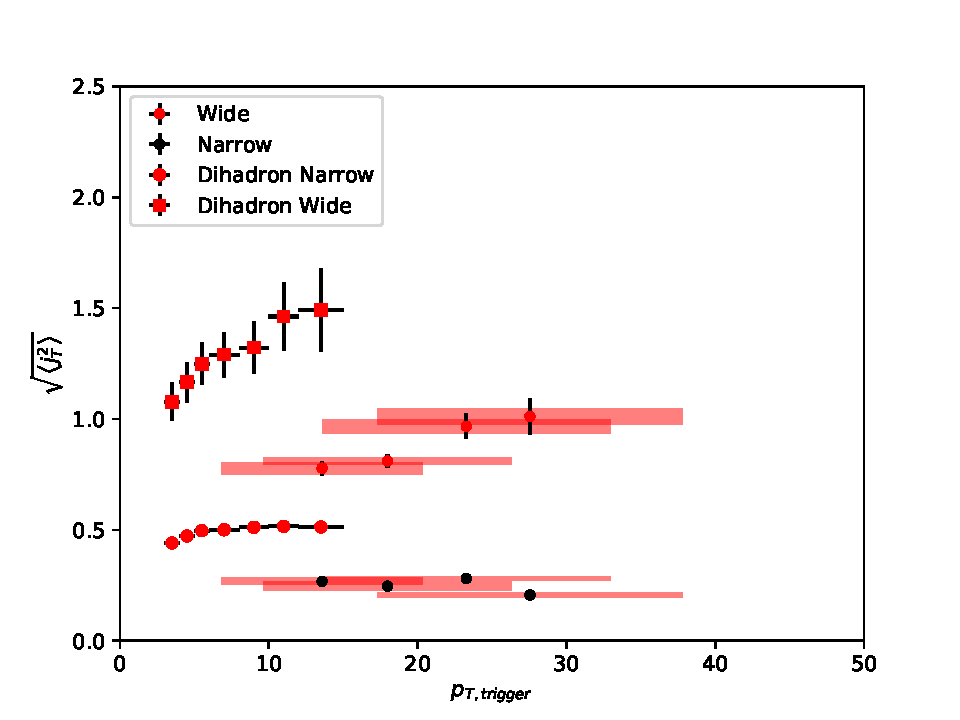
\includegraphics[width=0.99\textwidth]{figures/summary/RMSWithSystematics_DihadronTriggerPt.pdf}
\end{subfigure}
\begin{subfigure}{0.5\textwidth}
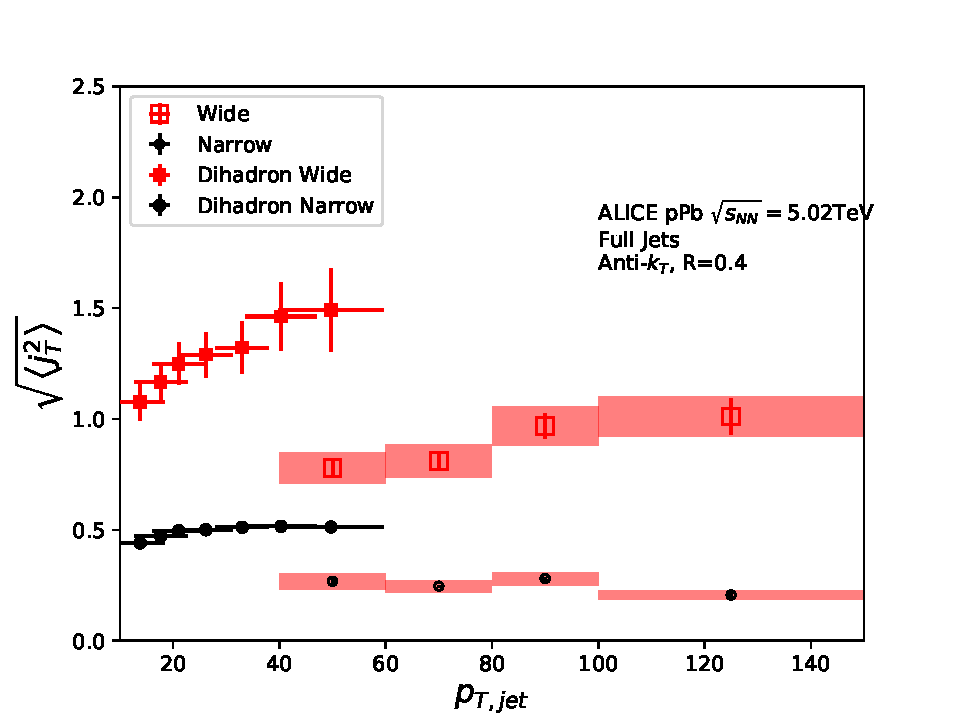
\includegraphics[width=0.99\textwidth]{figures/summary/RMSWithSystematics_DihadronJetPt.pdf}
\end{subfigure}
\caption{Jet $\jt{}$ results are compared to results obtained in the dihadron analysis. Dihadron trigger $\pt{}$ bins are converted to jet $\pt{}$  bins  using observed mean  $\pt{jet}$ values in $\pt{trigger}$ bins. Dihadron results are for $0.2 < x_{||} < 0.4$}
\label{fig:dihadroncomparison}
\end{figure}

\subsubsection{Different \texorpdfstring{$R$}{R} parameters}
\label{sec:Rstudy}
The size of the jet cone gives a limit for $\jt{}$. For a track with a fixed momentum $p$ this is a hard limit. This is conveniently seen as $\jt{}$ can be given in terms of cone size $R$ and momentum $p$ in the small angle approximation limit as

\begin{equation}
\jt{} \approx p \cdot R
\end{equation}

\noindent  Thus for tracks with $\pt{track} < \pt{0} $, $\jt{} < \pt{0} \times R$.
 

In practice the effect of cone sizes on $\jt{}$ distribution is studied in a \pythia~simulation. Results of the individual distributions and resulting RMS values from this simulation are shown in Fig.~\ref{fig:RcomparisonjT} and Fig.~\ref{fig:RcomparisonRMS} respectively. Increasing the cone size of jets gives more room for high $\jt{}$ tracks. This is seen in the individual $\jt{}$ distributions as increased high $\jt{}$ production. At low $\jt{}$ there is no change.

When looking at RMS values from wide component we see an increase/decrease of about 10\% when going from $R=0.4$ to $R=0.5$/$R=0.3$.

The message from narrow component RMS values is less clear. At low jet $\pt{}$ the behaviour is similar, but at high $\pt{}$ the order is reversed.
\begin{figure}[htp]
\centering
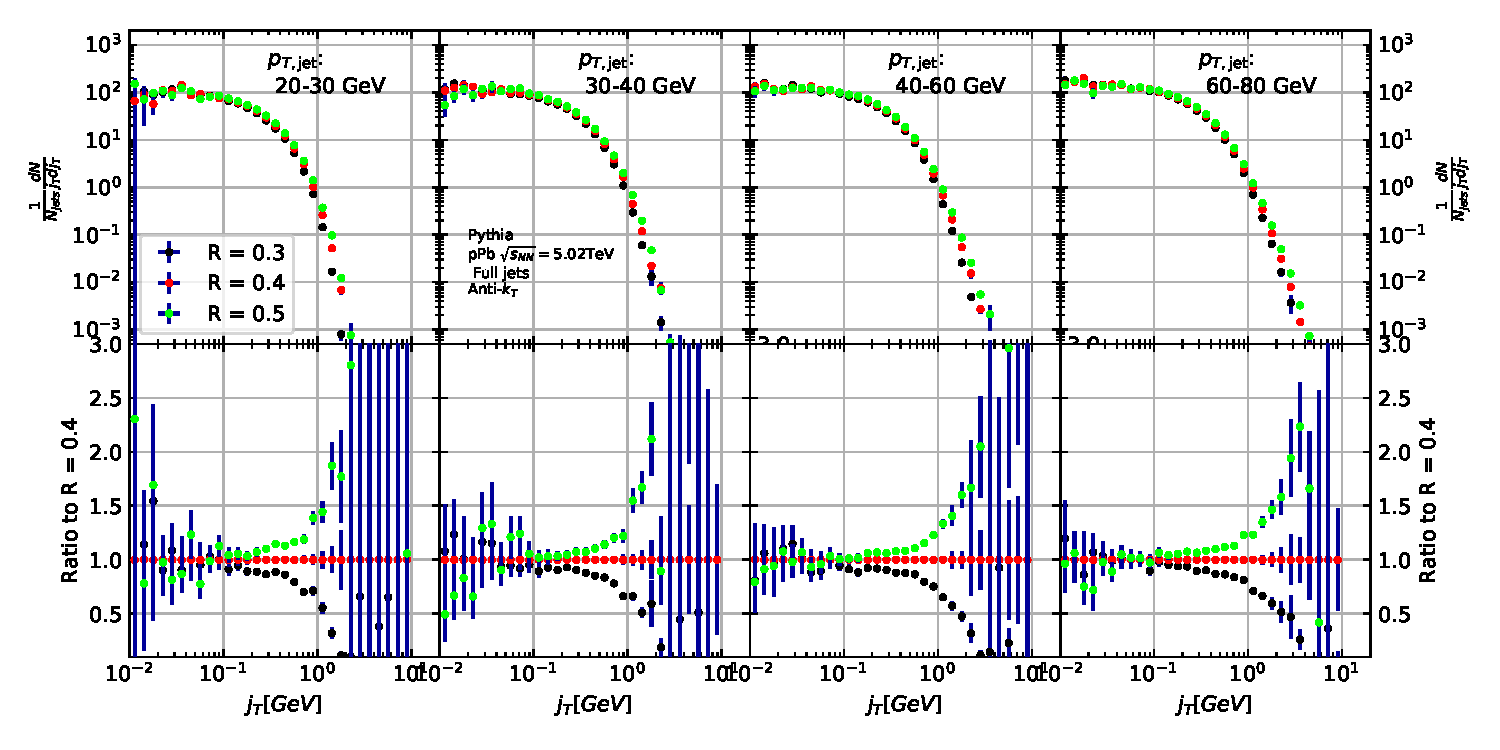
\includegraphics[width=0.8\textwidth]{results/RcomparisonSignal.pdf}
\caption[Pythia $R$ parameters $\jt{}$]{Effect of changing $R$ parameter in jet finding on $\jt{}$ distributions}
\label{fig:RcomparisonjT}
\end{figure}


\begin{figure}[htp]
\centering
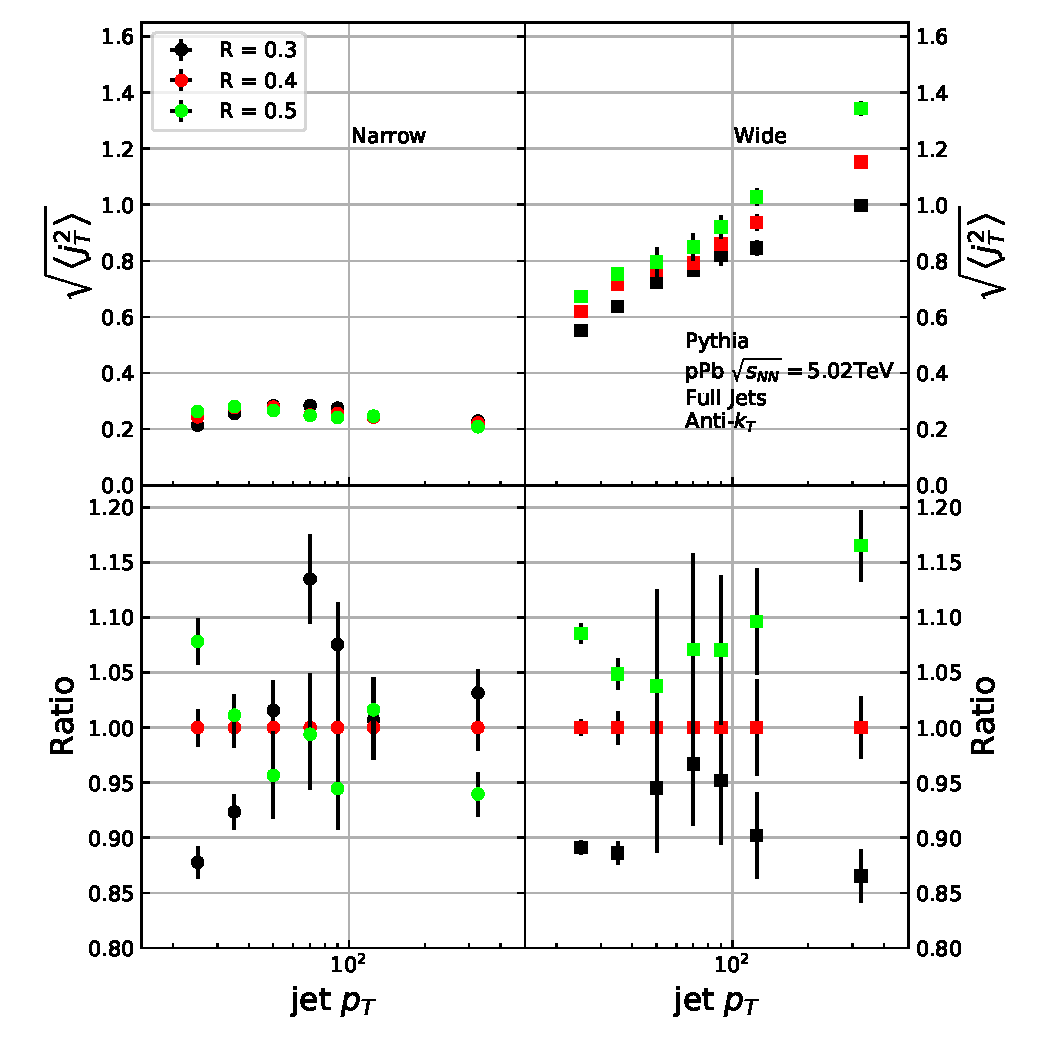
\includegraphics[width=0.6\textwidth]{figures/results/RcomparisonRMS.pdf} \\
\caption[Pythia $R$ parameters RMS]{Effect of changing $R$ parameter in jet finding on narrow and wide component RMS values. Wide component RMS values increase with increasing cone size.}
\label{fig:RcomparisonRMS}
\end{figure}


%Effect of the $R$ parameter choice is studied in \textsc{Pythia}. Having a fixed cone puts hard limits on the possible $\jt{}$ values. Increasing the cone size loosens these limits and allows higher $\jt{}$ values. The results are shown in Fig. \ref{fig:Rcomparison}. Left hand side shows the $\jt{}$ distributions. There is very little change in low $\jt{}$ but at high $\jt{}$ the yield increases. 

%This is also seen in the RMS values shown in the right hand side of Fig. \ref{fig:Rcomparison}, where the change in wide component RMS is about 10\% when going from $R=0.4$ to $R=0.3$ or $R=0.5$. With the narrow component values the situation is less clear. At low jet $\pt{}$ larger $R$ parameter leads to larger RMS values, but at high $\pt{jet}$ the situation is reversed; increasing the $R$ parameter decreases RMS values.

\subsubsection{Leading tracks versus jet}
\label{sec:reference}
The leading track is an imperfect estimate of the jet/original parton. Because the leading track in general is at an angle compared to the jet axis, the resulting $\jt{}$ values are different. In practice the jet axis found by the jet finding algrorithm tends to minimize the average $\jt{}$ of jet constituents. Thus the yield at high $\jt{}$ is limited and the RMS values are smaller.

A \textsc{Pythia} study was performed where $\jt{}$ was calculated with respect to the leading track momentum, instead of the jet axis. The results are shown in Fig. \ref{fig:RefComparison}. The resulting $\jt{}$ distributions are significantly wider than $\jt{}$ distributions from the typical method. The effect seems to be larger than the effect seen in comparing different $R$ values.

\begin{figure}[htp]
\centering
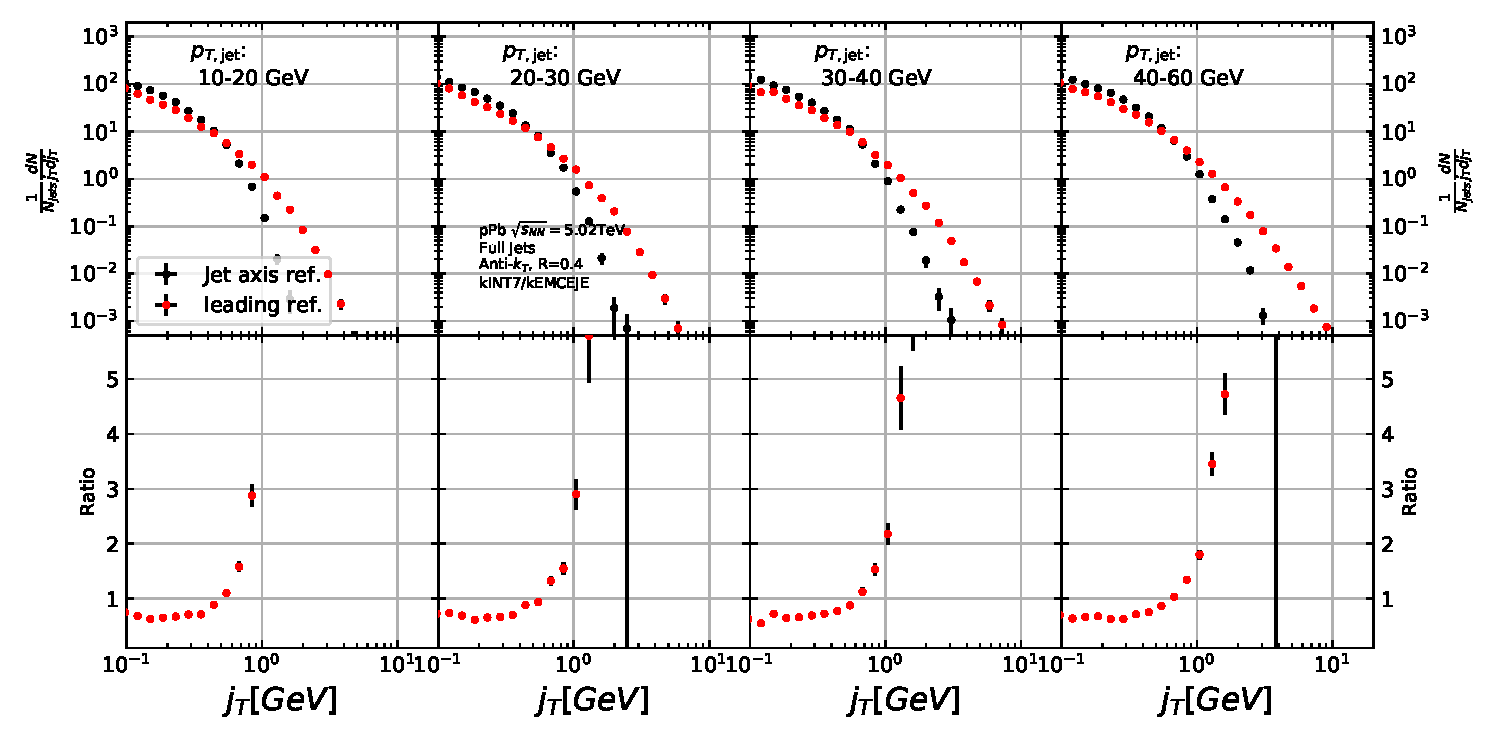
\includegraphics[width=0.55\textwidth]{figures/results/JetVsLeadingRefConst.pdf}
\caption{Results of calculating $\jt{}$ with respect to the jet axis or the leading hadron. The assumption is that because the leading hadron is an imperfect estimate of the jet axis, low $\jt{}$ tracks should on average be shifted to higher $\jt{}$}
\label{fig:RefComparison}
\end{figure}


\pagebreak
\FloatBarrier
\section{Summary}
\label{sec:sum}
In this work two distinct $\jt{}$ components were extracted for narrow and wide contributions using jet reconstruction in $\snn = \unit[5.02]{\tev}$ \pPb collisions. RMS values for both components were obtained. The width of the wide component is found to increase for increasing $\pt{jet}$. This is in part explained by the changing kinematical limits when going to higher $\pt{jet}$ which allows higher $\pt{track}$. Additionally the larger phase space allows stronger parton splitting. The results are qualitatively compatible with previous studies that studied $\jt{}$ using two-particle correlations.

{\color{red} Extend summary}
